\chapter{Resultados}
\label{cap:05}
\label{cap:resultados}

\section{Validação da Ferramenta GUY}
\label{sec:validacao_guy}

A validação inicial da ferramenta foi realizada com os arquivos de exemplo disponíveis em \texttt{src/examples/}. Os experimentos verificam se a extensão representa diferentes estruturas de controle em Python e se as métricas exibidas coincidem com uma reconstrução manual baseada na convenção da Seção \ref{sec:convencao_modelagem_gfc}. Todos os resultados apresentados nesta seção foram obtidos no modo de visualização simplificado.

Antes da execução, cada código foi percorrido manualmente para identificar comandos, decisões, pontos sintéticos e ligações de desvio. Dessa reconstrução foram obtidos \(N\), \(E\), o número de decisões e \(P\); em seguida, \(V(G)\) foi calculado de forma independente por \(E-N+2P\). O resultado foi classificado como conforme somente quando os valores esperados e exibidos coincidiram. A lista de caminhos foi conferida verificando-se início em \texttt{Entry}, término em \texttt{Exit}, validade das arestas e a introdução, por cada caminho adicional, de pelo menos uma aresta de decisão ainda não usada na base selecionada. Essa conferência caracteriza uma base operacional para os exemplos, não a enumeração de todos os caminhos de execução possíveis.

A Figura \ref{fig:vscode_grafo_GUY} apresenta apenas a organização geral do painel lateral usado durante a validação. As evidências específicas e legíveis de cada código são mostradas separadamente nas Figuras \ref{fig:gfc_experimento_i}, \ref{fig:gfc_experimento_ii} e \ref{fig:gfc_experimento_iii}; a captura introdutória não substitui essas três evidências.

\begin{figure}[H]
    \centering
    \caption{GFC gerado pelo GUY no VS Code.}
    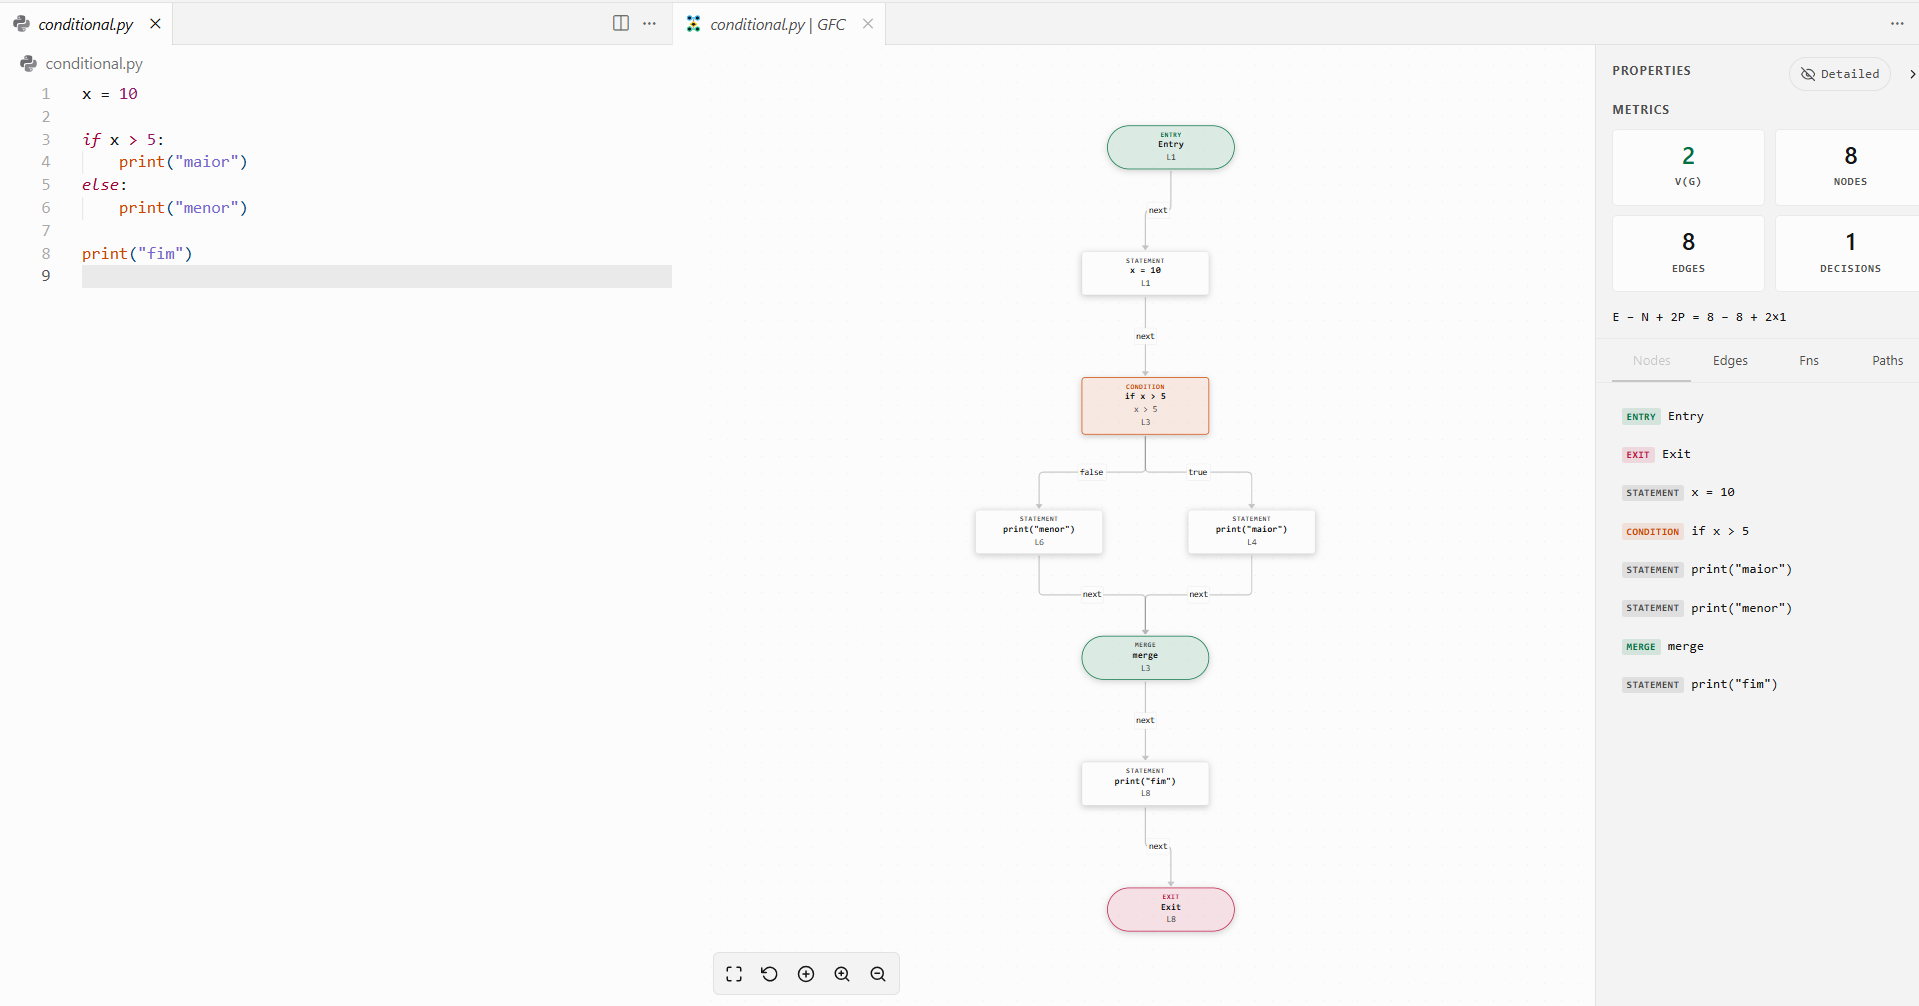
\includegraphics[width=0.85\linewidth]{imagens/ferramentas/guy-vscode.png}
    \fonte{Elaborada pelo autor.}
    \label{fig:vscode_grafo_GUY}
\end{figure}

\subsection{Experimento I: Código com Laço e Condicionais}

O primeiro experimento utiliza o arquivo \texttt{loop\_break\_continue.py}. O objetivo é verificar se a ferramenta representa corretamente um laço \texttt{while} contendo duas estruturas condicionais internas, uma com \texttt{continue} e outra com \texttt{break}. Esse cenário é importante porque envolve desvios que alteram o fluxo normal da iteração.

\begin{lstlisting}[language=Python, numbers=left, caption={Código utilizado no Experimento I.}, label={lst:experimento1_codigo}]
x = 0

while x < 10:
    x += 1
    if x == 3:
        continue
    if x == 8:
        break

print(x)
\end{lstlisting}

A Figura \ref{fig:gfc_experimento_i} apresenta o GFC produzido
pelo GUY para o código com laço, condicionais, \texttt{continue}
e \texttt{break}.

\begin{figure}[H]
    \centering
    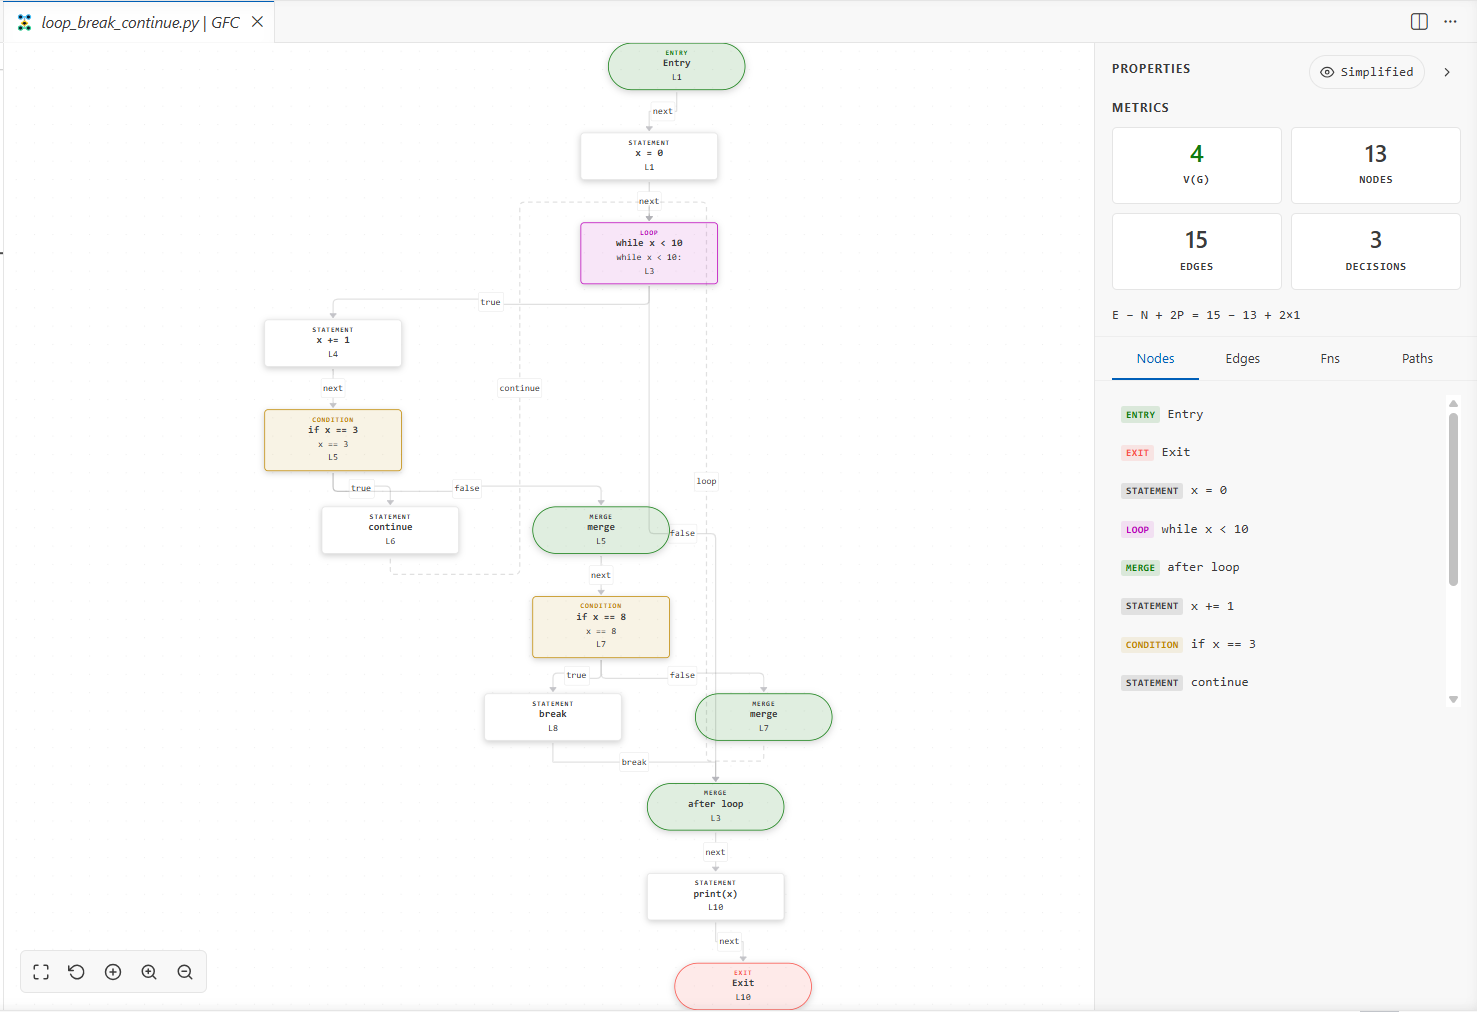
\includegraphics[
        width=\linewidth,
    ]{imagens/experimentos/gfc-experimento-i.png}
    \caption{GFC gerado pelo GUY no Experimento I.}
    \fonte{Elaborada pelo autor.}
    \label{fig:gfc_experimento_i}
\end{figure}

Ao analisar esse código, a ferramenta GUY identifica três pontos de decisão: a condição do \texttt{while} e os dois comandos \texttt{if}. O comando \texttt{continue} é representado por uma aresta que retorna para a condição do laço, enquanto o comando \texttt{break} é representado por uma aresta que conduz ao ponto posterior ao laço.

\begin{table}[H]
    \centering
    \caption{Comparação entre métricas esperadas e obtidas no Experimento I.}
    \begin{tabular}{l | c | c | c}
        \hline
        \textbf{Métrica} & \textbf{Esperado} & \textbf{Obtido} & \textbf{Status} \\ \hline
        Nós & 13 & 13 & Conforme \\ \hline
        Arestas & 15 & 15 & Conforme \\ \hline
        Decisões & 3 & 3 & Conforme \\ \hline
        Componentes & 1 & 1 & Conforme \\ \hline
        \(V(G)\) & 4 & 4 & Conforme \\ \hline
        Caminhos da base & 4 & 4 & Conforme \\ \hline
    \end{tabular}
    \fonte{Elaborada pelo autor.}
    \label{tab:experimento1_guy}
\end{table}

Na reconstrução manual foram contados: \texttt{Entry}; inicialização; condição do \texttt{while}; incremento; duas condições \texttt{if}; nós de \texttt{continue} e \texttt{break}; dois nós \texttt{merge}; \texttt{after loop}; impressão; e \texttt{Exit}, totalizando 13 nós. As 15 conexões incluem o retorno do \texttt{continue} à condição e a saída do \texttt{break} para \texttt{after loop}. Assim, \(V(G) = 15 - 13 + 2 \times 1 = 4\), resultado também compatível com três decisões acrescidas da região inicial para este grafo conectado.

\subsection{Experimento II: Código Condicional Simples}

O segundo experimento utiliza o arquivo \texttt{conditional.py}. O objetivo é validar o comportamento da ferramenta diante de uma estrutura condicional simples, composta por um \texttt{if}, um \texttt{else} e uma instrução executada após a junção dos dois ramos.

\begin{lstlisting}[language=Python, numbers=left, caption={Código utilizado no Experimento II.}, label={lst:experimento2_codigo}]
x = 10

if x > 5:
    print("maior")
else:
    print("menor")

print("fim")
\end{lstlisting}

Nesse caso, a ferramenta cria um nó de decisão para a condição \texttt{x > 5}, duas saídas para representar os ramos verdadeiro e falso e um nó de junção antes da continuidade do fluxo para o comando final.

A Figura \ref{fig:gfc_experimento_ii} apresenta o GFC produzido pelo GUY para o código com uma estrutura condicional simples, composta pelos fluxos verdadeiro e falso.

\begin{figure}[H]
    \centering
    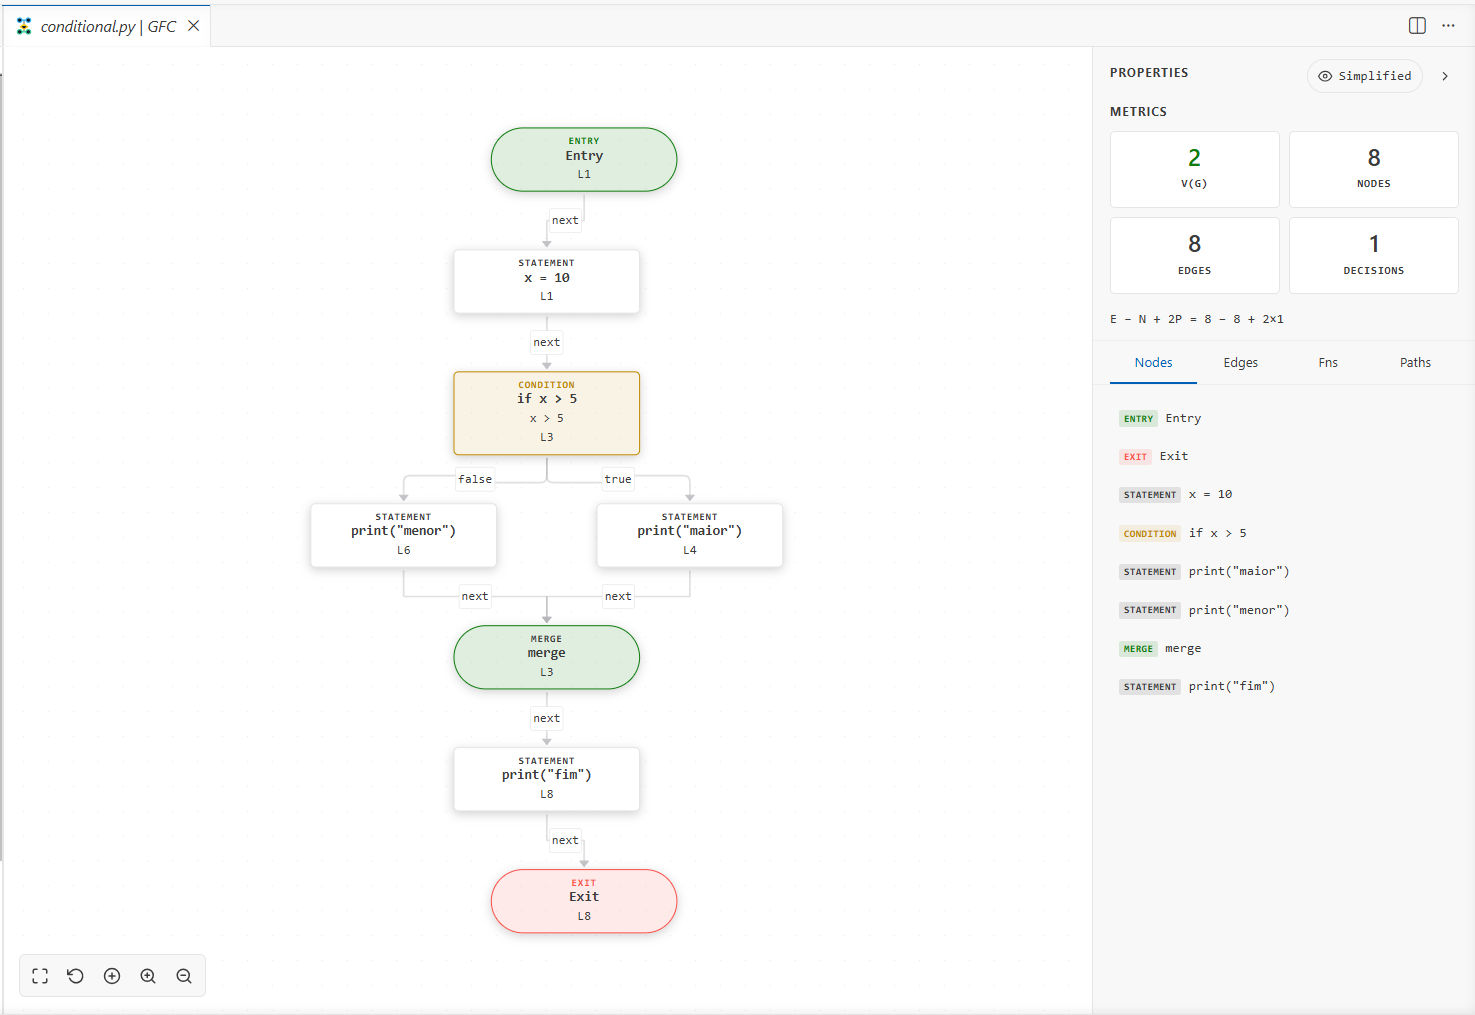
\includegraphics[
        width=\linewidth,
    ]{imagens/experimentos/gfc-experimento-ii.png}
    \caption{GFC gerado pelo GUY no Experimento II.}
    \fonte{Elaborada pelo autor.}
    \label{fig:gfc_experimento_ii}
\end{figure}

\begin{table}[H]
    \centering
    \caption{Comparação entre métricas esperadas e obtidas no Experimento II.}
    \begin{tabular}{l | c | c | c}
        \hline
        \textbf{Métrica} & \textbf{Esperado} & \textbf{Obtido} & \textbf{Status} \\ \hline
        Nós & 8 & 8 & Conforme \\ \hline
        Arestas & 8 & 8 & Conforme \\ \hline
        Decisões & 1 & 1 & Conforme \\ \hline
        Componentes & 1 & 1 & Conforme \\ \hline
        \(V(G)\) & 2 & 2 & Conforme \\ \hline
        Caminhos da base & 2 & 2 & Conforme \\ \hline
    \end{tabular}
    \fonte{Elaborada pelo autor.}
    \label{tab:experimento2_guy}
\end{table}

A Complexidade Ciclomática calculada é \(V(G) = 8 - 8 + 2 \times 1 = 2\), representando os dois fluxos possíveis de execução: o caminho em que a condição é verdadeira e o caminho em que ela é falsa.

\subsection{Experimento III: Código com Função, Laço e Condicional}

O terceiro experimento utiliza o arquivo \texttt{functions.py}, analisando especificamente a função \texttt{calculate\_total}. O objetivo é verificar o comando de geração do GFC a partir da função atual, bem como a representação combinada de laço \texttt{for}, condicional \texttt{if} e retorno de valor.

\begin{lstlisting}[language=Python, numbers=left, caption={Código utilizado no Experimento III.}, label={lst:experimento3_codigo}]
def calculate_total(items):
    total = 0
    for item in items:
        if item > 0:
            total += item
    return total
\end{lstlisting}

Ao posicionar o cursor dentro da função e executar o comando \texttt{GUY: Generate CFG from Current Function}, a extensão restringe a análise ao corpo da função selecionada. O grafo resultante contém a inicialização da variável, a condição de iteração do \texttt{for}, a decisão interna do \texttt{if}, o retorno ao laço e o comando \texttt{return} conectado ao nó de saída.

A Figura \ref{fig:gfc_experimento_iii} apresenta o GFC produzido pelo GUY para o código que combina declaração de função, laço de repetição e estrutura condicional.

\begin{figure}[H]
    \centering
    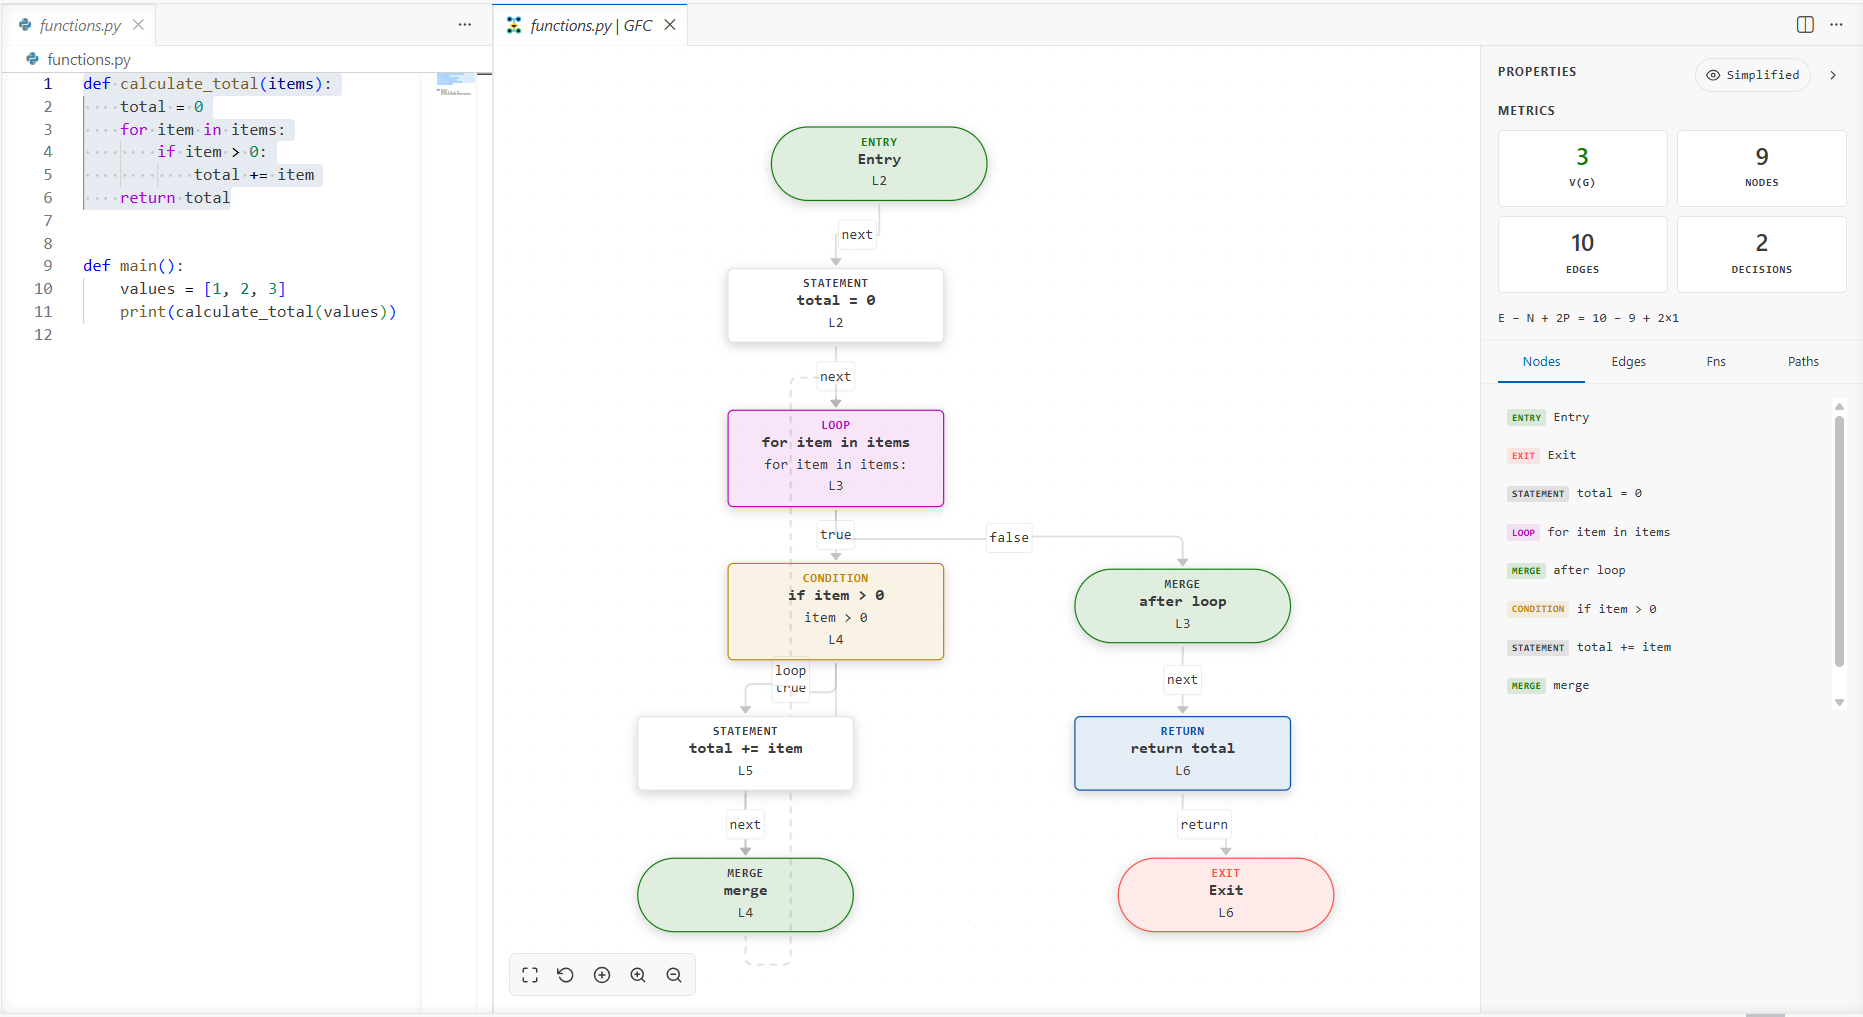
\includegraphics[
        width=\linewidth,
        trim={10 20 10 20},
        clip
    ]{imagens/experimentos/gfc-experimento-iii.png}
    \caption{GFC gerado pelo GUY no Experimento III.}
    \fonte{Elaborada pelo autor.}
    \label{fig:gfc_experimento_iii}
\end{figure}

\begin{table}[H]
    \centering
    \caption{Comparação entre métricas esperadas e obtidas no Experimento III.}
    \begin{tabular}{l | c | c | c}
        \hline
        \textbf{Métrica} & \textbf{Esperado} & \textbf{Obtido} & \textbf{Status} \\ \hline
        Nós & 9 & 9 & Conforme \\ \hline
        Arestas & 10 & 10 & Conforme \\ \hline
        Decisões & 2 & 2 & Conforme \\ \hline
        Componentes & 1 & 1 & Conforme \\ \hline
        \(V(G)\) & 3 & 3 & Conforme \\ \hline
        Caminhos da base & 3 & 3 & Conforme \\ \hline
    \end{tabular}
    \fonte{Elaborada pelo autor.}
    \label{tab:experimento3_guy}
\end{table}

A Complexidade Ciclomática calculada é \(V(G) = 10 - 9 + 2 \times 1 = 3\). O resultado reflete os dois pontos de decisão presentes na função: a repetição do \texttt{for} e a condição \texttt{if item > 0}. Os três caminhos selecionados formam uma base operacional para exercitar arestas de decisão distintas; isso não implica que três casos de teste sejam suficientes para satisfazer outros critérios de cobertura ou revelar todos os defeitos.

\section{Discussão dos Resultados e Limitações}

Os três experimentos demonstram, no conjunto limitado de exemplos selecionados, correspondência entre as estruturas Python analisadas, os grafos exibidos e o cálculo de Complexidade Ciclomática. Diferentemente das ferramentas correlatas examinadas, o protótipo apresenta a métrica junto ao GFC e mantém ligações entre seus elementos e os intervalos do código-fonte.

Como características observadas, a análise é acionada no VS Code, pode abranger arquivo, seleção ou função atual e é executada sem envio do código a um serviço mantido pelo GUY. Essa arquitetura elimina essa transmissão específica, mas não constitui, por si só, uma avaliação completa de segurança, privacidade ou usabilidade.

A seleção de nós, arestas e caminhos na Webview destaca as regiões correspondentes no editor. O modo simplificado reduz o número de elementos visuais ao condensar comandos sequenciais, enquanto o detalhado preserva maior granularidade. O efeito dessas funções sobre aprendizagem, produtividade ou facilidade de uso exige avaliação com usuários e não foi medido pelos experimentos técnicos.

Como limitação, a versão atual concentra-se em Python e em estruturas de controle comuns, como condicionais, laços, retornos, \texttt{break} e \texttt{continue}. Casos mais avançados da linguagem, como exceções, chamadas entre funções, recursão, geradores, programação assíncrona e efeitos dinâmicos de execução, ainda não são representados de forma completa. Além disso, por se tratar de análise estática, a ferramenta não substitui a execução de testes nem garante a identificação de todos os comportamentos possíveis em tempo de execução.

Também há limitações relacionadas à visualização de grafos muito grandes. Embora a interface apresente avisos e o sistema oculte a listagem de caminhos independentes em grafos extensos para manter a responsividade, programas com muitas estruturas aninhadas podem gerar representações visualmente densas. Nesses casos, a análise por seleção ou por função tende a ser mais adequada do que a análise do arquivo completo.

Os resultados sustentam somente as estruturas e os três cenários efetivamente apresentados. Casos-limite, entradas inválidas, equivalência entre modos e comportamento sob grafos extensos precisam de uma matriz de testes própria antes de ampliar essas conclusões. As recomendações de evolução são consolidadas no Capítulo \ref{cap:conclusoes}.
